%%%%%%%%%%%%%%%%%%%%%%%%%%%%%%%%%%%%%%%%%%%%%%%%%%%%%%%%%%%%
% 2.9 ARITHMETIC GEOMETRY
% The Composition of Advanced Mathematics
%%%%%%%%%%%%%%%%%%%%%%%%%%%%%%%%%%%%%%%%%%%%%%%%%%%%%%%%%%%%

\section{Arithmetic Geometry}
\label{sec:arithmetic-geometry}

\prerequisite{
Algebraic Number Theory from \cref{sec:algebraic-number-theory},
Diophantine Geometry from \cref{sec:diophantine-geometry},
and familiarity with fields, rings, ideals, polynomial equations,
rational points, elliptic curves, and finite fields. Algebraic Geometry
is developed canonically in Chapter 3; this section introduces the
arithmetic viewpoint without duplicating its full geometric machinery.
}

\learningobjectives{
By the end of this section, the reader should be able to:
\begin{itemize}
    \item explain the central goals of arithmetic geometry;
    \item interpret polynomial equations as geometric objects over different fields;
    \item distinguish rational, integral, finite-field, real, and \(p\)-adic points;
    \item explain why changing the base field changes the arithmetic problem;
    \item understand the local--global viewpoint;
    \item explain reduction modulo primes;
    \item distinguish good and bad reduction for elliptic curves;
    \item compute simple point counts over finite fields;
    \item state Hasse's bound for elliptic curves;
    \item explain how local point counts produce global arithmetic information;
    \item understand the basic role of elliptic-curve \(L\)-functions;
    \item state the Mordell--Weil theorem in the arithmetic-geometric setting;
    \item distinguish torsion and rank;
    \item explain the purpose of height functions;
    \item understand the canonical height on elliptic curves;
    \item explain the basic idea of descent;
    \item describe the role of the Tate--Shafarevich group conceptually;
    \item state the Birch and Swinnerton-Dyer conjecture conceptually;
    \item explain the role of modularity in the arithmetic of elliptic curves;
    \item understand how Fermat's Last Theorem fits into arithmetic geometry;
    \item explain why higher-genus curves lead naturally to Jacobians;
    \item state Faltings's theorem;
    \item explain the role of abelian varieties;
    \item recognize schemes as a framework that unifies geometry over fields
    and arithmetic over rings;
    \item understand why \(\operatorname{Spec}\Z\) behaves geometrically;
    \item explain the analogy between prime numbers and geometric points;
    \item understand arithmetic surfaces conceptually;
    \item recognize the importance of zeta functions and \(L\)-functions;
    \item connect arithmetic geometry with algebraic geometry, number theory,
    analysis, topology, and representation theory.
\end{itemize}
}

%%%%%%%%%%%%%%%%%%%%%%%%%%%%%%%%%%%%%%%%%%%%%%%%%%%%%%%%%%%%
\subsection{What Is Arithmetic Geometry?}
\label{subsec:what-is-arithmetic-geometry}
%%%%%%%%%%%%%%%%%%%%%%%%%%%%%%%%%%%%%%%%%%%%%%%%%%%%%%%%%%%%

Arithmetic geometry studies polynomial equations using both number theory
and geometry.

The central objects are algebraic varieties defined over arithmetic fields
and rings such as

\[ \Q,\qquad \Z,\qquad \F_p,\qquad \Q_p, \]

and number fields.

The subject asks questions such as:

\begin{itemize}
    \item Does a variety have rational points?
    \item Does it have integer points?
    \item How many points does it have modulo a prime?
    \item How are its points distributed?
    \item How does its geometry control its arithmetic?
    \item How does arithmetic change when the base field changes?
\end{itemize}

\begin{definitionbox}{Arithmetic Geometry}
\emph{Arithmetic geometry} is the study of algebraic geometric objects
together with arithmetic properties of their points, equations, and
associated invariants.
\end{definitionbox}

A guiding principle is

\[
\boxed{
\text{Number Theory}
+
\text{Algebraic Geometry}
=
\text{Arithmetic Geometry}.
}
\]

%%%%%%%%%%%%%%%%%%%%%%%%%%%%%%%%%%%%%%%%%%%%%%%%%%%%%%%%%%%%
\subsection{The Arithmetic-Geometric Viewpoint}
\label{subsec:arithmetic-geometric-viewpoint}
%%%%%%%%%%%%%%%%%%%%%%%%%%%%%%%%%%%%%%%%%%%%%%%%%%%%%%%%%%%%

Consider a polynomial equation

\[ F(x_1,\ldots,x_n)=0. \]

The same equation can be studied over many different number systems:

\[
\R,\qquad
\C,\qquad
\Q,\qquad
\Q_p,\qquad
\F_p.
\]

Geometrically, the equation defines an algebraic object.

Arithmetically, we ask which points on that object have coordinates in the
chosen number system.

Thus the equation is fixed while the arithmetic environment changes.

%%%%%%%%%%%%%%%%%%%%%%%%%%%%%%%%%%%%%%%%%%%%%%%%%%%%%%%%%%%%
\subsection{Points Over Different Fields}
\label{subsec:points-over-different-fields}
%%%%%%%%%%%%%%%%%%%%%%%%%%%%%%%%%%%%%%%%%%%%%%%%%%%%%%%%%%%%

Let \(X\) be an algebraic variety.

The notation

\[ X(K) \]

means the set of points of \(X\) whose coordinates lie in the field \(K\).

It is read ``the \(K\)-points of \(X\)'' or ``the points of \(X\) over
\(K\).''

Important examples are

\[
X(\Q),\qquad
X(\R),\qquad
X(\C),\qquad
X(\Q_p),\qquad
X(\F_p).
\]

Each set can reveal different information about the same geometric object.

%%%%%%%%%%%%%%%%%%%%%%%%%%%%%%%%%%%%%%%%%%%%%%%%%%%%%%%%%%%%
\subsection{A Simple Example}
\label{subsec:arithmetic-geometry-simple-example}
%%%%%%%%%%%%%%%%%%%%%%%%%%%%%%%%%%%%%%%%%%%%%%%%%%%%%%%%%%%%

Consider

\[ X:x^2+y^2=1. \]

Over \(\R\), this is the ordinary unit circle.

Over \(\Q\), we ask for rational points such as

\[ \left(\frac35,\frac45\right). \]

Over \(\F_5\), we solve

\[ x^2+y^2\equiv1\pmod5. \]

Thus one equation produces several related arithmetic problems.

%%%%%%%%%%%%%%%%%%%%%%%%%%%%%%%%%%%%%%%%%%%%%%%%%%%%%%%%%%%%
\subsection{The Base Field Matters}
\label{subsec:base-field-matters}
%%%%%%%%%%%%%%%%%%%%%%%%%%%%%%%%%%%%%%%%%%%%%%%%%%%%%%%%%%%%

An equation may have solutions over one field but not another.

For example,

\[ x^2+1=0 \]

has no solution in \(\R\), but it has solutions

\[ x=\pm i \]

in \(\C\).

Likewise, an equation may have real solutions but no rational solutions.

Therefore:

\[
\boxed{
X(K)\text{ depends essentially on the field }K.
}
\]

Changing the base field is one of the basic operations of arithmetic
geometry.

%%%%%%%%%%%%%%%%%%%%%%%%%%%%%%%%%%%%%%%%%%%%%%%%%%%%%%%%%%%%
\subsection{Local and Global Arithmetic}
\label{subsec:local-global-arithmetic-geometry}
%%%%%%%%%%%%%%%%%%%%%%%%%%%%%%%%%%%%%%%%%%%%%%%%%%%%%%%%%%%%

The rational numbers form the global field

\[ \Q. \]

Arithmetic problems over \(\Q\) can be studied locally using

\[
\R
\qquad\text{and}\qquad
\Q_p
\]

for every prime \(p\).

Thus one compares

\[ X(\Q) \]

with

\[ X(\R),\qquad X(\Q_2),\qquad X(\Q_3),\qquad X(\Q_5),\ldots \]

This produces the local--global viewpoint.

%%%%%%%%%%%%%%%%%%%%%%%%%%%%%%%%%%%%%%%%%%%%%%%%%%%%%%%%%%%%
\subsection{Local Obstructions}
\label{subsec:local-obstructions-arithmetic-geometry}
%%%%%%%%%%%%%%%%%%%%%%%%%%%%%%%%%%%%%%%%%%%%%%%%%%%%%%%%%%%%

If

\[ X(\Q)=\varnothing, \]

one possible explanation is that \(X\) already has no points over some local
field.

For example,

\[ X(\Q_p)=\varnothing \]

for a particular prime \(p\) immediately implies

\[ X(\Q)=\varnothing. \]

Likewise,

\[ X(\R)=\varnothing \]

implies there are no rational points.

Thus local fields provide efficient tests for global impossibility.

%%%%%%%%%%%%%%%%%%%%%%%%%%%%%%%%%%%%%%%%%%%%%%%%%%%%%%%%%%%%
\subsection{Local Solvability Is Not Always Enough}
\label{subsec:local-not-always-global}
%%%%%%%%%%%%%%%%%%%%%%%%%%%%%%%%%%%%%%%%%%%%%%%%%%%%%%%%%%%%

One might hope that

\[
X(\R)\neq\varnothing
\quad\text{and}\quad
X(\Q_p)\neq\varnothing
\text{ for every }p
\]

would imply

\[ X(\Q)\neq\varnothing. \]

This is true for important classes of equations but false in general.

Failures of this principle are among the central phenomena of arithmetic
geometry.

\begin{conceptbox}
Local arithmetic can detect many global obstructions, but global rational
points may contain information invisible at every individual local field.
\end{conceptbox}

%%%%%%%%%%%%%%%%%%%%%%%%%%%%%%%%%%%%%%%%%%%%%%%%%%%%%%%%%%%%
\subsection{Reduction Modulo Primes}
\label{subsec:reduction-modulo-primes-arithmetic-geometry}
%%%%%%%%%%%%%%%%%%%%%%%%%%%%%%%%%%%%%%%%%%%%%%%%%%%%%%%%%%%%

Suppose an equation has integer coefficients.

Reducing those coefficients modulo a prime \(p\) produces an equation over

\[ \F_p. \]

For example,

\[ y^2=x^3-x+1 \]

becomes the same formal equation interpreted modulo \(p\).

This process is called \emph{reduction modulo \(p\)}.

It converts an infinite arithmetic problem into one over a finite field.

%%%%%%%%%%%%%%%%%%%%%%%%%%%%%%%%%%%%%%%%%%%%%%%%%%%%%%%%%%%%
\subsection{Why Finite Fields Help}
\label{subsec:why-finite-fields-help-arithmetic-geometry}
%%%%%%%%%%%%%%%%%%%%%%%%%%%%%%%%%%%%%%%%%%%%%%%%%%%%%%%%%%%%

The field

\[ \F_p \]

contains only \(p\) elements.

Therefore every possible coordinate can, in principle, be checked.

Finite-field point counts reveal information about:

\begin{itemize}
    \item local solvability;
    \item torsion;
    \item reduction behavior;
    \item zeta functions;
    \item \(L\)-functions;
    \item Galois representations;
    \item cryptographic groups.
\end{itemize}

Arithmetic geometry repeatedly extracts global information from such local
finite data.

%%%%%%%%%%%%%%%%%%%%%%%%%%%%%%%%%%%%%%%%%%%%%%%%%%%%%%%%%%%%
\subsection{Worked Example: A Curve Modulo \(5\)}
\label{subsec:worked-curve-mod-five}
%%%%%%%%%%%%%%%%%%%%%%%%%%%%%%%%%%%%%%%%%%%%%%%%%%%%%%%%%%%%

Consider

\[ E:y^2=x^3-x+1. \]

We determine its points over

\[ \F_5. \]

The quadratic residues modulo \(5\) are

\[ 0,\qquad1,\qquad4. \]

\begin{workedexamplebox}{Counting \(E(\F_5)\)}

\begin{tabularx}{\textwidth}{@{}>{\raggedright\arraybackslash}p{0.35\textwidth}X@{}}
\(x=0\) & \(x^3-x+1\equiv1\), giving \(y=\pm1\)\\
\(x=1\) & \(x^3-x+1\equiv1\), giving \(y=\pm1\)\\
\(x=2\) & \(x^3-x+1\equiv2\), giving no \(y\)\\
\(x=3\) & \(x^3-x+1\equiv0\), giving \(y=0\)\\
\(x=4\) & \(x^3-x+1\equiv1\), giving \(y=\pm1\)
\end{tabularx}

There are

\[ 2+2+0+1+2=7 \]

affine points.

Including the point at infinity gives

\begin{answerbox}
\[ \boxed{\#E(\F_5)=8.} \]
\end{answerbox}
\end{workedexamplebox}

%%%%%%%%%%%%%%%%%%%%%%%%%%%%%%%%%%%%%%%%%%%%%%%%%%%%%%%%%%%%
\subsection{Point Counting Table}
\label{subsec:point-counting-table}
%%%%%%%%%%%%%%%%%%%%%%%%%%%%%%%%%%%%%%%%%%%%%%%%%%%%%%%%%%%%

The preceding computation can be organized compactly:

\[
\begin{array}{c|c|c}
x & x^3-x+1\pmod5 & \text{number of }y\\
\hline
0 & 1 & 2\\
1 & 1 & 2\\
2 & 2 & 0\\
3 & 0 & 1\\
4 & 1 & 2
\end{array}
\]

Thus

\[ \#E(\F_5)=7+1=8, \]

where the final \(1\) accounts for the point at infinity.

%%%%%%%%%%%%%%%%%%%%%%%%%%%%%%%%%%%%%%%%%%%%%%%%%%%%%%%%%%%%
\subsection{Good and Bad Reduction}
\label{subsec:good-bad-reduction}
%%%%%%%%%%%%%%%%%%%%%%%%%%%%%%%%%%%%%%%%%%%%%%%%%%%%%%%%%%%%

Consider an elliptic curve

\[ E:y^2=x^3+Ax+B. \]

Its discriminant is

\[ \boxed{\Delta=-16(4A^3+27B^2).} \]

The capital Greek letter

\[ \Delta \]

is \emph{Delta}, pronounced ``delta.''

The curve is nonsingular when

\[ \Delta\neq0. \]

After reduction modulo \(p\), the curve may remain nonsingular or become
singular.

%%%%%%%%%%%%%%%%%%%%%%%%%%%%%%%%%%%%%%%%%%%%%%%%%%%%%%%%%%%%
\subsection{Good Reduction}
\label{subsec:good-reduction}
%%%%%%%%%%%%%%%%%%%%%%%%%%%%%%%%%%%%%%%%%%%%%%%%%%%%%%%%%%%%

\begin{definitionbox}{Good Reduction}
An elliptic curve has \emph{good reduction} at a prime \(p\) when its
reduction modulo \(p\) remains nonsingular.
\end{definitionbox}

For an integral Weierstrass model, primes not dividing the discriminant are
good candidates for good reduction.

Conceptually,

\[ p\nmid\Delta \]

means the geometry survives reduction cleanly.

%%%%%%%%%%%%%%%%%%%%%%%%%%%%%%%%%%%%%%%%%%%%%%%%%%%%%%%%%%%%
\subsection{Bad Reduction}
\label{subsec:bad-reduction}
%%%%%%%%%%%%%%%%%%%%%%%%%%%%%%%%%%%%%%%%%%%%%%%%%%%%%%%%%%%%

\begin{definitionbox}{Bad Reduction}
An elliptic curve has \emph{bad reduction} at \(p\) when its reduction modulo
\(p\) becomes singular.
\end{definitionbox}

For an integral Weierstrass model, bad reduction can occur only at primes
dividing the discriminant.

Thus only finitely many primes are bad.

This finite exceptional set plays an important role in arithmetic invariants
attached to the curve.

%%%%%%%%%%%%%%%%%%%%%%%%%%%%%%%%%%%%%%%%%%%%%%%%%%%%%%%%%%%%
\subsection{Reduction Visual}
\label{subsec:reduction-visual}
%%%%%%%%%%%%%%%%%%%%%%%%%%%%%%%%%%%%%%%%%%%%%%%%%%%%%%%%%%%%

\begin{centereddiagram}
\begin{tikzpicture}[
node distance=1.6cm and 1.8cm,
every node/.style={draw,rounded corners,align=center,inner sep=6pt}
]
\node (Q) {Elliptic curve\\over \(\Q\)};
\node[below left=of Q] (good) {reduction mod \(p\)\\nonsingular};
\node[below right=of Q] (bad) {reduction mod \(p\)\\singular};
\node[below=of good] (G) {good reduction};
\node[below=of bad] (B) {bad reduction};

\draw[-{Latex[length=2.2mm]}] (Q)--(good);
\draw[-{Latex[length=2.2mm]}] (Q)--(bad);
\draw[-{Latex[length=2.2mm]}] (good)--(G);
\draw[-{Latex[length=2.2mm]}] (bad)--(B);
\end{tikzpicture}
\end{centereddiagram}

%%%%%%%%%%%%%%%%%%%%%%%%%%%%%%%%%%%%%%%%%%%%%%%%%%%%%%%%%%%%
\subsection{Hasse's Bound}
\label{subsec:hasse-bound-arithmetic-geometry}
%%%%%%%%%%%%%%%%%%%%%%%%%%%%%%%%%%%%%%%%%%%%%%%%%%%%%%%%%%%%

For a prime of good reduction, write

\[ \#E(\F_p)=p+1-a_p. \]

The quantity \(a_p\) is called the \emph{trace of Frobenius} at \(p\).

\begin{theorem}[Hasse]
For an elliptic curve over \(\F_p\),

\[ \boxed{|a_p|\leq2\sqrt p.} \]
\end{theorem}

Equivalently,

\[ \boxed{p+1-2\sqrt p\leq\#E(\F_p)\leq p+1+2\sqrt p.} \]

Thus elliptic curves over finite fields have approximately \(p+1\) points.

%%%%%%%%%%%%%%%%%%%%%%%%%%%%%%%%%%%%%%%%%%%%%%%%%%%%%%%%%%%%
\subsection{Worked Example: Hasse's Bound}
\label{subsec:worked-hasse-bound}
%%%%%%%%%%%%%%%%%%%%%%%%%%%%%%%%%%%%%%%%%%%%%%%%%%%%%%%%%%%%

\begin{workedexamplebox}{Bounding \(\#E(\F_{11})\)}

Hasse's theorem gives

\[ |\#E(\F_{11})-12|\leq2\sqrt{11}. \]

Since

\[ 2\sqrt{11}\approx6.63, \]

we obtain

\[ 5.37\lesssim\#E(\F_{11})\lesssim18.63. \]

The number of points is an integer.

\begin{answerbox}
\[ \boxed{6\leq\#E(\F_{11})\leq18.} \]
\end{answerbox}
\end{workedexamplebox}

%%%%%%%%%%%%%%%%%%%%%%%%%%%%%%%%%%%%%%%%%%%%%%%%%%%%%%%%%%%%
\subsection{Frobenius}
\label{subsec:frobenius-arithmetic-geometry}
%%%%%%%%%%%%%%%%%%%%%%%%%%%%%%%%%%%%%%%%%%%%%%%%%%%%%%%%%%%%

Over the finite field \(\F_p\), the map

\[ x\longmapsto x^p \]

is called the \emph{Frobenius map}.

For elements of \(\F_p\),

\[ x^p=x. \]

Over larger finite fields, Frobenius remains a fundamental symmetry.

In arithmetic geometry, Frobenius acts on algebraic objects and associated
cohomological structures.

Its traces and eigenvalues encode point-counting information.

%%%%%%%%%%%%%%%%%%%%%%%%%%%%%%%%%%%%%%%%%%%%%%%%%%%%%%%%%%%%
\subsection{From Point Counts to Arithmetic Data}
\label{subsec:point-counts-arithmetic-data}
%%%%%%%%%%%%%%%%%%%%%%%%%%%%%%%%%%%%%%%%%%%%%%%%%%%%%%%%%%%%

For an elliptic curve, the values

\[ a_p=p+1-\#E(\F_p) \]

vary with \(p\).

A sequence such as

\[ a_2,a_3,a_5,a_7,a_{11},\ldots \]

contains substantial information about the original curve over \(\Q\).

This is one of the remarkable principles of arithmetic geometry:

\[
\boxed{
\text{finite-field shadows}
\longrightarrow
\text{global arithmetic information}.
}
\]

%%%%%%%%%%%%%%%%%%%%%%%%%%%%%%%%%%%%%%%%%%%%%%%%%%%%%%%%%%%%
\subsection{Elliptic-Curve \(L\)-Functions}
\label{subsec:elliptic-l-function-arithmetic-geometry}
%%%%%%%%%%%%%%%%%%%%%%%%%%%%%%%%%%%%%%%%%%%%%%%%%%%%%%%%%%%%

For primes of good reduction, the local factor associated with \(p\) is

\[ \frac{1}{1-a_pp^{-s}+p^{1-2s}}. \]

These factors are assembled into an Euler product defining the elliptic-curve
\(L\)-function

\[ L(E,s). \]

Schematically,

\[ \boxed{L(E,s)=\prod_p L_p(E,s).} \]

The precise local factors at bad primes require separate treatment.

%%%%%%%%%%%%%%%%%%%%%%%%%%%%%%%%%%%%%%%%%%%%%%%%%%%%%%%%%%%%
\subsection{Local Data and Global Functions}
\label{subsec:local-data-global-functions}
%%%%%%%%%%%%%%%%%%%%%%%%%%%%%%%%%%%%%%%%%%%%%%%%%%%%%%%%%%%%

The construction of \(L(E,s)\) follows a recurring number-theoretic pattern:

\[
\boxed{
\text{data at each prime}
\longrightarrow
\text{Euler product}
\longrightarrow
\text{global analytic object}.
}
\]

The Riemann zeta function follows the same philosophy:

\[ \zeta(s)=\prod_p\frac1{1-p^{-s}}. \]

Arithmetic geometry generalizes this idea to geometric objects.

%%%%%%%%%%%%%%%%%%%%%%%%%%%%%%%%%%%%%%%%%%%%%%%%%%%%%%%%%%%%
\subsection{Rational Points on Elliptic Curves}
\label{subsec:rational-points-elliptic-arithmetic}
%%%%%%%%%%%%%%%%%%%%%%%%%%%%%%%%%%%%%%%%%%%%%%%%%%%%%%%%%%%%

An elliptic curve over \(\Q\) has a group of rational points

\[ E(\Q). \]

The Mordell--Weil theorem states:

\begin{theorem}[Mordell--Weil]
The group \(E(\Q)\) is finitely generated.
\end{theorem}

Therefore

\[ \boxed{E(\Q)\cong E(\Q)_{\mathrm{tors}}\oplus\Z^r.} \]

The finite group

\[ E(\Q)_{\mathrm{tors}} \]

contains the torsion points.

The integer \(r\) is the rank.

%%%%%%%%%%%%%%%%%%%%%%%%%%%%%%%%%%%%%%%%%%%%%%%%%%%%%%%%%%%%
\subsection{Why Rank Matters}
\label{subsec:why-rank-matters-arithmetic}
%%%%%%%%%%%%%%%%%%%%%%%%%%%%%%%%%%%%%%%%%%%%%%%%%%%%%%%%%%%%

Rank measures the number of independent rational points of infinite order.

If

\[ r=0, \]

then \(E(\Q)\) is finite.

If

\[ r>0, \]

then \(E(\Q)\) is infinite.

Thus determining the rank is a fundamental rational-point problem.

Unfortunately, the Mordell--Weil theorem does not by itself provide a simple
general formula for \(r\).

%%%%%%%%%%%%%%%%%%%%%%%%%%%%%%%%%%%%%%%%%%%%%%%%%%%%%%%%%%%%
\subsection{Height Functions}
\label{subsec:height-arithmetic-geometry}
%%%%%%%%%%%%%%%%%%%%%%%%%%%%%%%%%%%%%%%%%%%%%%%%%%%%%%%%%%%%

Rational points can have coordinates with increasingly large numerators and
denominators.

Height functions measure this arithmetic complexity.

For a rational number

\[ x=\frac ab \]

in lowest terms, a basic height is

\[ H(x)=\max\{|a|,|b|\}. \]

For projective points and varieties, height functions generalize this
measurement.

%%%%%%%%%%%%%%%%%%%%%%%%%%%%%%%%%%%%%%%%%%%%%%%%%%%%%%%%%%%%
\subsection{Canonical Height}
\label{subsec:canonical-height-arithmetic-geometry}
%%%%%%%%%%%%%%%%%%%%%%%%%%%%%%%%%%%%%%%%%%%%%%%%%%%%%%%%%%%%

Elliptic curves possess a refined height

\[ \hat h(P), \]

called the \emph{canonical height}.

It satisfies

\[ \boxed{\hat h(nP)=n^2\hat h(P).} \]

This property matches the group structure of the elliptic curve.

For a non-torsion point \(P\),

\[ \hat h(P)>0. \]

For torsion points,

\[ \hat h(P)=0. \]

Thus the canonical height helps distinguish finite-order and infinite-order
behavior.

%%%%%%%%%%%%%%%%%%%%%%%%%%%%%%%%%%%%%%%%%%%%%%%%%%%%%%%%%%%%
\subsection{Arithmetic Size and Geometry}
\label{subsec:arithmetic-size-geometry}
%%%%%%%%%%%%%%%%%%%%%%%%%%%%%%%%%%%%%%%%%%%%%%%%%%%%%%%%%%%%

Height provides a bridge between geometry and arithmetic.

Geometrically, points lie on the same curve.

Arithmetically, their coordinates may have vastly different complexity.

One can therefore study questions such as:

\[ \#\{P\in X(\Q):H(P)\leq B\}. \]

This counts rational points of bounded arithmetic size.

Such counting problems are central in modern arithmetic geometry.

%%%%%%%%%%%%%%%%%%%%%%%%%%%%%%%%%%%%%%%%%%%%%%%%%%%%%%%%%%%%
\subsection{Descent}
\label{subsec:descent-arithmetic-geometry}
%%%%%%%%%%%%%%%%%%%%%%%%%%%%%%%%%%%%%%%%%%%%%%%%%%%%%%%%%%%%

A major method for studying rational points is \emph{descent}.

The basic philosophy is to map a difficult rational-point problem into a
simpler auxiliary arithmetic problem.

For elliptic curves, descent can provide information about

\[ E(\Q)/nE(\Q). \]

The quotient records rational points modulo multiplication by \(n\).

Common examples include:

\[
2\text{-descent},\qquad
3\text{-descent},\qquad
n\text{-descent}.
\]

%%%%%%%%%%%%%%%%%%%%%%%%%%%%%%%%%%%%%%%%%%%%%%%%%%%%%%%%%%%%
\subsection{The Descent Philosophy}
\label{subsec:descent-philosophy}
%%%%%%%%%%%%%%%%%%%%%%%%%%%%%%%%%%%%%%%%%%%%%%%%%%%%%%%%%%%%

The method can be represented schematically as

\[
\boxed{
E(\Q)
\longrightarrow
\text{finite auxiliary arithmetic data}
\longrightarrow
\text{information about rank and rational points}.
}
\]

Descent does not usually list all rational points immediately.

Instead, it converts an infinite problem into finite algebraic calculations
and local-solvability tests.

%%%%%%%%%%%%%%%%%%%%%%%%%%%%%%%%%%%%%%%%%%%%%%%%%%%%%%%%%%%%
\subsection{Selmer Groups}
\label{subsec:selmer-groups-introduction}
%%%%%%%%%%%%%%%%%%%%%%%%%%%%%%%%%%%%%%%%%%%%%%%%%%%%%%%%%%%%

Descent naturally produces groups called \emph{Selmer groups}.

For multiplication by an integer \(n\), one encounters the \(n\)-Selmer
group, written

\[ \operatorname{Sel}^{(n)}(E/\Q). \]

The notation is read ``the \(n\)-Selmer group of \(E\) over \(\Q\).''

Conceptually, a Selmer group combines:

\begin{itemize}
    \item global algebraic information;
    \item local solvability conditions;
    \item finite computable data.
\end{itemize}

Selmer groups can provide upper bounds for the Mordell--Weil rank.

%%%%%%%%%%%%%%%%%%%%%%%%%%%%%%%%%%%%%%%%%%%%%%%%%%%%%%%%%%%%
\subsection{Tate--Shafarevich Group}
\label{subsec:tate-shafarevich-group}
%%%%%%%%%%%%%%%%%%%%%%%%%%%%%%%%%%%%%%%%%%%%%%%%%%%%%%%%%%%%

An important object measuring failures of local--global reasoning is the
Tate--Shafarevich group.

It is commonly written

\[ \Sha(E/\Q). \]

The symbol

\[ \Sha \]

is the Cyrillic letter \emph{Sha}, pronounced ``shah.''

Conceptually, \(\Sha(E/\Q)\) records certain objects associated with \(E\)
that have points everywhere locally but fail to have rational points
globally.

%%%%%%%%%%%%%%%%%%%%%%%%%%%%%%%%%%%%%%%%%%%%%%%%%%%%%%%%%%%%
\subsection{Why \(\Sha\) Matters}
\label{subsec:why-sha-matters}
%%%%%%%%%%%%%%%%%%%%%%%%%%%%%%%%%%%%%%%%%%%%%%%%%%%%%%%%%%%%

The Tate--Shafarevich group lies precisely at the boundary between local and
global arithmetic.

Very roughly,

\[
\boxed{
\text{locally solvable everywhere}
\quad\text{but}\quad
\text{globally obstructed}
}
\]

is the phenomenon it helps measure for torsors under elliptic curves.

Its finiteness is itself a major open problem in general.

%%%%%%%%%%%%%%%%%%%%%%%%%%%%%%%%%%%%%%%%%%%%%%%%%%%%%%%%%%%%
\subsection{Birch and Swinnerton-Dyer}
\label{subsec:bsd-arithmetic-geometry}
%%%%%%%%%%%%%%%%%%%%%%%%%%%%%%%%%%%%%%%%%%%%%%%%%%%%%%%%%%%%

The Birch and Swinnerton-Dyer conjecture connects rational points with the
analytic behavior of the elliptic-curve \(L\)-function.

\begin{conjecture}[Birch and Swinnerton-Dyer]
For an elliptic curve \(E/\Q\),

\[ \boxed{\operatorname{rank}E(\Q)=\operatorname{ord}_{s=1}L(E,s).} \]
\end{conjecture}

The notation

\[ \operatorname{ord}_{s=1}L(E,s) \]

means the order of vanishing of \(L(E,s)\) at \(s=1\).

%%%%%%%%%%%%%%%%%%%%%%%%%%%%%%%%%%%%%%%%%%%%%%%%%%%%%%%%%%%%
\subsection{Algebraic and Analytic Rank}
\label{subsec:algebraic-analytic-rank}
%%%%%%%%%%%%%%%%%%%%%%%%%%%%%%%%%%%%%%%%%%%%%%%%%%%%%%%%%%%%

The quantity

\[ \operatorname{rank}E(\Q) \]

is called the \emph{algebraic rank}.

The quantity

\[ \operatorname{ord}_{s=1}L(E,s) \]

is called the \emph{analytic rank}.

BSD predicts

\[ \boxed{\text{algebraic rank}=\text{analytic rank}.} \]

Thus a group of rational solutions would be controlled by the zero of a
complex analytic function.

%%%%%%%%%%%%%%%%%%%%%%%%%%%%%%%%%%%%%%%%%%%%%%%%%%%%%%%%%%%%
\subsection{The Refined BSD Philosophy}
\label{subsec:refined-bsd-philosophy}
%%%%%%%%%%%%%%%%%%%%%%%%%%%%%%%%%%%%%%%%%%%%%%%%%%%%%%%%%%%%

The full Birch and Swinnerton-Dyer conjecture predicts much more than the
equality of ranks.

The leading behavior of \(L(E,s)\) near \(s=1\) is expected to encode
arithmetic invariants including:

\begin{itemize}
    \item the torsion subgroup;
    \item a regulator built from canonical heights;
    \item local arithmetic factors;
    \item the Tate--Shafarevich group;
    \item additional arithmetic data associated with \(E\).
\end{itemize}

Thus the conjecture proposes a remarkably detailed dictionary between
analysis and arithmetic.

%%%%%%%%%%%%%%%%%%%%%%%%%%%%%%%%%%%%%%%%%%%%%%%%%%%%%%%%%%%%
\subsection{Arithmetic-Analytic Bridge}
\label{subsec:arithmetic-analytic-bridge}
%%%%%%%%%%%%%%%%%%%%%%%%%%%%%%%%%%%%%%%%%%%%%%%%%%%%%%%%%%%%

\begin{centereddiagram}
\begin{tikzpicture}[
node distance=1.4cm and 1.4cm,
every node/.style={draw,rounded corners,align=center,inner sep=6pt}
]
\node (E) {Elliptic curve\\\(E/\Q\)};
\node[right=of E] (Fp) {point counts\\\(\#E(\F_p)\)};
\node[right=of Fp] (ap) {coefficients\\\(a_p\)};
\node[below=of ap] (L) {\(L\)-function\\\(L(E,s)\)};
\node[left=of L] (BSD) {behavior at\\\(s=1\)};
\node[left=of BSD] (R) {rank of\\\(E(\Q)\)};

\draw[-{Latex[length=2.2mm]}] (E)--(Fp);
\draw[-{Latex[length=2.2mm]}] (Fp)--(ap);
\draw[-{Latex[length=2.2mm]}] (ap)--(L);
\draw[-{Latex[length=2.2mm]}] (L)--(BSD);
\draw[-{Latex[length=2.2mm]}] (BSD)--(R);
\end{tikzpicture}
\end{centereddiagram}

The final arrow is conjectural in the full generality predicted by BSD.

%%%%%%%%%%%%%%%%%%%%%%%%%%%%%%%%%%%%%%%%%%%%%%%%%%%%%%%%%%%%
\subsection{Modularity of Elliptic Curves}
\label{subsec:modularity-arithmetic-geometry}
%%%%%%%%%%%%%%%%%%%%%%%%%%%%%%%%%%%%%%%%%%%%%%%%%%%%%%%%%%%%

A major theorem states that every elliptic curve over \(\Q\) is modular.

Very roughly, there exists a modular form whose arithmetic coefficients
match the data of the elliptic curve.

Schematically,

\[ \boxed{E/\Q\longleftrightarrow\text{modular form}.} \]

This correspondence provides analytic continuation and a functional equation
for the \(L\)-function of the elliptic curve.

%%%%%%%%%%%%%%%%%%%%%%%%%%%%%%%%%%%%%%%%%%%%%%%%%%%%%%%%%%%%
\subsection{Why Modularity Is Remarkable}
\label{subsec:why-modularity-remarkable}
%%%%%%%%%%%%%%%%%%%%%%%%%%%%%%%%%%%%%%%%%%%%%%%%%%%%%%%%%%%%

An elliptic curve begins as an algebraic equation such as

\[ y^2=x^3+Ax+B. \]

A modular form is an analytic function possessing strong symmetry
properties.

Modularity therefore connects two objects that initially appear unrelated:

\[
\boxed{
\text{algebraic geometry}
\longleftrightarrow
\text{complex analysis}.
}
\]

The matching arithmetic data reveals that they encode the same deeper
structure.

%%%%%%%%%%%%%%%%%%%%%%%%%%%%%%%%%%%%%%%%%%%%%%%%%%%%%%%%%%%%
\subsection{Fermat's Last Theorem}
\label{subsec:flt-arithmetic-geometry}
%%%%%%%%%%%%%%%%%%%%%%%%%%%%%%%%%%%%%%%%%%%%%%%%%%%%%%%%%%%%

Fermat's Last Theorem states that

\[ x^n+y^n=z^n \]

has no positive integer solutions for

\[ n>2. \]

Its modern proof is a landmark application of arithmetic geometry.

The key strategy was not to attack the Fermat equation directly.

Instead, a hypothetical solution was used to construct an elliptic curve.

%%%%%%%%%%%%%%%%%%%%%%%%%%%%%%%%%%%%%%%%%%%%%%%%%%%%%%%%%%%%
\subsection{The Frey Curve Strategy}
\label{subsec:frey-curve-strategy-arithmetic}
%%%%%%%%%%%%%%%%%%%%%%%%%%%%%%%%%%%%%%%%%%%%%%%%%%%%%%%%%%%%

A hypothetical nontrivial solution to an appropriate Fermat equation leads
to an elliptic curve of the general form

\[ y^2=x(x-a^n)(x+b^n). \]

This Frey curve would possess highly unusual arithmetic properties.

Deep results concerning modularity imply that such a curve cannot exist.

Therefore the hypothetical Fermat solution cannot exist.

Schematically,

\[
\boxed{
\text{Fermat solution}
\Longrightarrow
\text{Frey curve}
\Longrightarrow
\text{impossible modular behavior}
\Longrightarrow
\text{contradiction}.
}
\]

%%%%%%%%%%%%%%%%%%%%%%%%%%%%%%%%%%%%%%%%%%%%%%%%%%%%%%%%%%%%
\subsection{Higher-Genus Curves}
\label{subsec:higher-genus-arithmetic-geometry}
%%%%%%%%%%%%%%%%%%%%%%%%%%%%%%%%%%%%%%%%%%%%%%%%%%%%%%%%%%%%

Elliptic curves have genus \(1\).

For curves of genus

\[ g\geq2, \]

the rational-point problem changes dramatically.

Faltings's theorem gives:

\begin{theorem}[Faltings]
Let \(C\) be a smooth projective curve of genus \(g\geq2\) over a number
field \(K\). Then

\[ \boxed{C(K)\text{ is finite}.} \]
\end{theorem}

This theorem proves finiteness but does not automatically provide a complete
list of the rational points.

%%%%%%%%%%%%%%%%%%%%%%%%%%%%%%%%%%%%%%%%%%%%%%%%%%%%%%%%%%%%
\subsection{From Curves to Jacobians}
\label{subsec:curves-to-jacobians-arithmetic}
%%%%%%%%%%%%%%%%%%%%%%%%%%%%%%%%%%%%%%%%%%%%%%%%%%%%%%%%%%%%

A higher-genus curve generally lacks an intrinsic group law like that of an
elliptic curve.

Instead, one associates an abelian variety called its \emph{Jacobian}.

For a curve \(C\), write

\[ J(C). \]

The Jacobian has a group of rational points

\[ J(C)(\Q). \]

The curve can often be embedded into its Jacobian after choosing a suitable
base point.

%%%%%%%%%%%%%%%%%%%%%%%%%%%%%%%%%%%%%%%%%%%%%%%%%%%%%%%%%%%%
\subsection{Why Jacobians Help}
\label{subsec:why-jacobians-help}
%%%%%%%%%%%%%%%%%%%%%%%%%%%%%%%%%%%%%%%%%%%%%%%%%%%%%%%%%%%%

The Jacobian converts a rational-point problem on a curve into a group
problem on an abelian variety.

The Mordell--Weil theorem generalizes:

\begin{theorem}
If \(A\) is an abelian variety over a number field \(K\), then

\[ A(K) \]

is a finitely generated abelian group.
\end{theorem}

Thus higher-genus curves can be studied using the arithmetic of their
Jacobians.

%%%%%%%%%%%%%%%%%%%%%%%%%%%%%%%%%%%%%%%%%%%%%%%%%%%%%%%%%%%%
\subsection{Chabauty's Idea}
\label{subsec:chabauty-arithmetic-geometry}
%%%%%%%%%%%%%%%%%%%%%%%%%%%%%%%%%%%%%%%%%%%%%%%%%%%%%%%%%%%%

Suppose \(C\) is a curve of genus \(g\geq2\), and its Jacobian \(J\) has
Mordell--Weil rank \(r\).

When

\[ r<g, \]

Chabauty's method can often be used to control the rational points of \(C\).

Coleman's refinement uses \(p\)-adic integration to produce explicit bounds.

Conceptually,

\[
\boxed{
\text{low Jacobian rank}
+
\text{\(p\)-adic analysis}
\Longrightarrow
\text{strong restrictions on }C(\Q).
}
\]

%%%%%%%%%%%%%%%%%%%%%%%%%%%%%%%%%%%%%%%%%%%%%%%%%%%%%%%%%%%%
\subsection{Abelian Varieties}
\label{subsec:abelian-varieties-arithmetic-geometry}
%%%%%%%%%%%%%%%%%%%%%%%%%%%%%%%%%%%%%%%%%%%%%%%%%%%%%%%%%%%%

An elliptic curve is a one-dimensional abelian variety.

Higher-dimensional abelian varieties generalize elliptic curves while
retaining a compatible commutative group law.

They are central because they combine:

\begin{itemize}
    \item projective geometry;
    \item algebraic groups;
    \item number fields;
    \item height theory;
    \item Galois representations;
    \item \(L\)-functions.
\end{itemize}

Jacobians provide one of the most important sources of abelian varieties.

%%%%%%%%%%%%%%%%%%%%%%%%%%%%%%%%%%%%%%%%%%%%%%%%%%%%%%%%%%%%
\subsection{Why Ordinary Varieties Are Not Enough}
\label{subsec:why-schemes-arithmetic}
%%%%%%%%%%%%%%%%%%%%%%%%%%%%%%%%%%%%%%%%%%%%%%%%%%%%%%%%%%%%

Classical algebraic varieties are naturally defined over fields.

Arithmetic, however, often requires working over rings such as

\[ \Z. \]

For example, we may want to study one equation simultaneously over

\[
\Q,\qquad
\F_2,\qquad
\F_3,\qquad
\F_5,\ldots
\]

rather than treating every prime separately.

This motivates the language of schemes.

%%%%%%%%%%%%%%%%%%%%%%%%%%%%%%%%%%%%%%%%%%%%%%%%%%%%%%%%%%%%
\subsection{The Spectrum of a Ring}
\label{subsec:spectrum-ring-arithmetic}
%%%%%%%%%%%%%%%%%%%%%%%%%%%%%%%%%%%%%%%%%%%%%%%%%%%%%%%%%%%%

For a commutative ring \(R\), the notation

\[ \Spec(R) \]

denotes the set of prime ideals of \(R\) equipped with additional geometric
structure.

The notation is read ``spectrum of \(R\).''

This construction allows commutative rings to be treated geometrically.

The full theory belongs canonically to Algebraic Geometry.

Here we focus on its arithmetic meaning.

%%%%%%%%%%%%%%%%%%%%%%%%%%%%%%%%%%%%%%%%%%%%%%%%%%%%%%%%%%%%
\subsection{The Geometry of \(\Spec(\Z)\)}
\label{subsec:geometry-spec-z}
%%%%%%%%%%%%%%%%%%%%%%%%%%%%%%%%%%%%%%%%%%%%%%%%%%%%%%%%%%%%

The prime ideals of \(\Z\) are

\[ (0) \]

and

\[ (p) \]

for each prime number \(p\).

Thus the points of

\[ \Spec(\Z) \]

include

\[
(2),\qquad
(3),\qquad
(5),\qquad
(7),\ldots
\]

together with the generic point \((0)\).

Prime numbers therefore appear literally as geometric points.

%%%%%%%%%%%%%%%%%%%%%%%%%%%%%%%%%%%%%%%%%%%%%%%%%%%%%%%%%%%%
\subsection{\(\Spec(\Z)\) Visual}
\label{subsec:spec-z-visual}
%%%%%%%%%%%%%%%%%%%%%%%%%%%%%%%%%%%%%%%%%%%%%%%%%%%%%%%%%%%%

\begin{centereddiagram}
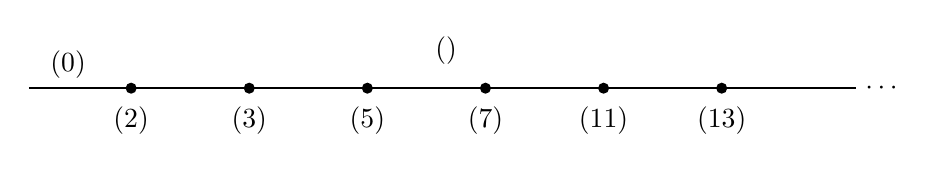
\begin{tikzpicture}
\draw[thick] (-0.3,0)--(10.2,0);

\foreach \x/\p in {1/2,2.5/3,4/5,5.5/7,7/11,8.5/13}{
    \fill (\x,0) circle (2pt);
    \node[below=3pt] at (\x,0) {\((\p)\)};
}

\node[above=5pt] at (5,0) {\(\Spec(\Z)\)};
\node[right] at (10.2,0) {\(\cdots\)};
\node[above] at (0.2,0) {\((0)\)};
\end{tikzpicture}
\end{centereddiagram}

This picture is schematic, but it captures the arithmetic analogy:
primes behave like geometric locations.

%%%%%%%%%%%%%%%%%%%%%%%%%%%%%%%%%%%%%%%%%%%%%%%%%%%%%%%%%%%%
\subsection{Fibers Over Primes}
\label{subsec:fibers-over-primes}
%%%%%%%%%%%%%%%%%%%%%%%%%%%%%%%%%%%%%%%%%%%%%%%%%%%%%%%%%%%%

Suppose an arithmetic geometric object \(X\) is defined over \(\Z\).

There is conceptually a map

\[ X\longrightarrow\Spec(\Z). \]

Above each prime point

\[ (p) \]

lies the reduction of \(X\) modulo \(p\).

This reduction is called the \emph{fiber at \(p\)}.

Above the generic point lies the characteristic-zero object, often viewed
over \(\Q\).

%%%%%%%%%%%%%%%%%%%%%%%%%%%%%%%%%%%%%%%%%%%%%%%%%%%%%%%%%%%%
\subsection{Arithmetic Fibers Visual}
\label{subsec:arithmetic-fibers-visual}
%%%%%%%%%%%%%%%%%%%%%%%%%%%%%%%%%%%%%%%%%%%%%%%%%%%%%%%%%%%%

\begin{centereddiagram}
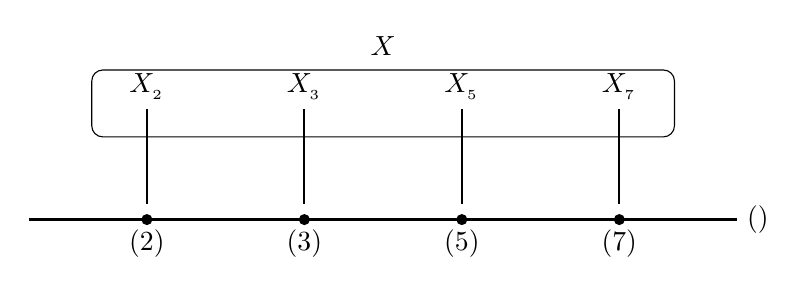
\begin{tikzpicture}
\draw[thick] (0,0)--(9,0);
\node[right] at (9,0) {\(\Spec(\Z)\)};

\foreach \x/\p in {1.5/2,3.5/3,5.5/5,7.5/7}{
    \fill (\x,0) circle (2pt);
    \node[below] at (\x,0) {\((\p)\)};
    \draw[thick] (\x,0.2)--(\x,1.4);
    \node[above] at (\x,1.4) {\(X_{\F_\p}\)};
}

\node at (4.5,2.2) {\(X\)};
\draw[rounded corners] (0.8,1.05) rectangle (8.2,1.9);
\end{tikzpicture}
\end{centereddiagram}

The notation

\[ X_{\F_p} \]

is read ``\(X\) over \(\F_p\)'' and represents the fiber obtained by
reduction modulo \(p\).

%%%%%%%%%%%%%%%%%%%%%%%%%%%%%%%%%%%%%%%%%%%%%%%%%%%%%%%%%%%%
\subsection{Arithmetic Surfaces}
\label{subsec:arithmetic-surfaces}
%%%%%%%%%%%%%%%%%%%%%%%%%%%%%%%%%%%%%%%%%%%%%%%%%%%%%%%%%%%%

A curve varying over

\[ \Spec(\Z) \]

behaves like a two-dimensional geometric object.

Such objects motivate the term \emph{arithmetic surface}.

One direction corresponds roughly to the geometry of the curve.

The other corresponds to arithmetic variation across primes.

This viewpoint turns prime-by-prime arithmetic into geometry over a common
base.

%%%%%%%%%%%%%%%%%%%%%%%%%%%%%%%%%%%%%%%%%%%%%%%%%%%%%%%%%%%%
\subsection{Prime Numbers as Geometric Places}
\label{subsec:primes-as-geometric-places}
%%%%%%%%%%%%%%%%%%%%%%%%%%%%%%%%%%%%%%%%%%%%%%%%%%%%%%%%%%%%

Arithmetic geometry develops a powerful analogy:

\[
\boxed{
\text{prime numbers}
\longleftrightarrow
\text{geometric points or places}.
}
\]

Reducing modulo \(p\) becomes analogous to examining what happens over a
specific geometric location.

This explains why terms such as

\begin{itemize}
    \item local;
    \item fiber;
    \item ramification;
    \item divisor;
    \item intersection;
\end{itemize}

appear naturally in number theory.

%%%%%%%%%%%%%%%%%%%%%%%%%%%%%%%%%%%%%%%%%%%%%%%%%%%%%%%%%%%%
\subsection{Number Fields as Arithmetic Curves}
\label{subsec:number-fields-arithmetic-curves}
%%%%%%%%%%%%%%%%%%%%%%%%%%%%%%%%%%%%%%%%%%%%%%%%%%%%%%%%%%%%

Let \(K\) be a number field with ring of integers

\[ \mathcal O_K. \]

The scheme

\[ \Spec(\mathcal O_K) \]

can be viewed as an arithmetic analogue of a curve.

Its prime ideals behave like points.

Ramification of primes in number fields then acquires a geometric
interpretation.

Thus algebraic number theory itself can be reinterpreted geometrically.

%%%%%%%%%%%%%%%%%%%%%%%%%%%%%%%%%%%%%%%%%%%%%%%%%%%%%%%%%%%%
\subsection{Ramification Revisited}
\label{subsec:ramification-arithmetic-geometry}
%%%%%%%%%%%%%%%%%%%%%%%%%%%%%%%%%%%%%%%%%%%%%%%%%%%%%%%%%%%%

Suppose a rational prime \(p\) factors in a number field as

\[ p\mathcal O_K=\mathfrak p_1^{e_1}\cdots\mathfrak p_g^{e_g}. \]

The exponents

\[ e_1,\ldots,e_g \]

are ramification indices.

Geometrically, ramification describes how the map

\[ \Spec(\mathcal O_K)\longrightarrow\Spec(\Z) \]

behaves above the point \((p)\).

Thus prime factorization becomes geometric branching.

%%%%%%%%%%%%%%%%%%%%%%%%%%%%%%%%%%%%%%%%%%%%%%%%%%%%%%%%%%%%
\subsection{Ramification Visual}
\label{subsec:ramification-visual-arithmetic}
%%%%%%%%%%%%%%%%%%%%%%%%%%%%%%%%%%%%%%%%%%%%%%%%%%%%%%%%%%%%

\begin{centereddiagram}
\begin{tikzpicture}
\node[draw,circle,inner sep=2pt] (p) at (0,0) {\(p\)};
\node[draw,circle,inner sep=2pt] (p1) at (-2,1.8) {\(\mathfrak p_1\)};
\node[draw,circle,inner sep=2pt] (p2) at (0,1.8) {\(\mathfrak p_2\)};
\node[draw,circle,inner sep=2pt] (p3) at (2,1.8) {\(\mathfrak p_3\)};

\draw[-{Latex[length=2.2mm]}] (p1)--(p);
\draw[-{Latex[length=2.2mm]}] (p2)--(p);
\draw[-{Latex[length=2.2mm]}] (p3)--(p);

\node[left] at (-2,1.8) {\scriptsize primes above \(p\)};
\end{tikzpicture}
\end{centereddiagram}

This geometric language becomes especially powerful in more advanced
arithmetic settings.

%%%%%%%%%%%%%%%%%%%%%%%%%%%%%%%%%%%%%%%%%%%%%%%%%%%%%%%%%%%%
\subsection{Zeta Functions of Varieties}
\label{subsec:zeta-functions-varieties}
%%%%%%%%%%%%%%%%%%%%%%%%%%%%%%%%%%%%%%%%%%%%%%%%%%%%%%%%%%%%

For a variety \(X\) over a finite field \(\F_q\), one can count points over
the extensions

\[ \F_q,\qquad\F_{q^2},\qquad\F_{q^3},\ldots \]

Let

\[ N_n=\#X(\F_{q^n}). \]

The local zeta function is defined by

\[ \boxed{
Z(X,T)=
\exp\left(
\sum_{n=1}^{\infty}\frac{N_nT^n}{n}
\right).
} \]

This function packages all finite-extension point counts into one generating
object.

%%%%%%%%%%%%%%%%%%%%%%%%%%%%%%%%%%%%%%%%%%%%%%%%%%%%%%%%%%%%
\subsection{Point Counts Become Functions}
\label{subsec:point-counts-become-functions}
%%%%%%%%%%%%%%%%%%%%%%%%%%%%%%%%%%%%%%%%%%%%%%%%%%%%%%%%%%%%

The construction

\[
N_1,N_2,N_3,\ldots
\]

becomes

\[ Z(X,T). \]

Thus arithmetic geometry repeatedly converts discrete counting information
into algebraic or analytic functions.

This is analogous to generating functions in combinatorics and Dirichlet
series in analytic number theory.

%%%%%%%%%%%%%%%%%%%%%%%%%%%%%%%%%%%%%%%%%%%%%%%%%%%%%%%%%%%%
\subsection{The Weil Conjectures}
\label{subsec:weil-conjectures-overview}
%%%%%%%%%%%%%%%%%%%%%%%%%%%%%%%%%%%%%%%%%%%%%%%%%%%%%%%%%%%%

The zeta functions of varieties over finite fields satisfy remarkable
structural properties.

These were predicted by the Weil conjectures and later proved.

Conceptually, they assert that \(Z(X,T)\):

\begin{itemize}
    \item is a rational function;
    \item satisfies a functional equation;
    \item has zeros and poles governed by geometric invariants;
    \item satisfies an analogue of the Riemann Hypothesis.
\end{itemize}

The proofs required the development of powerful cohomological machinery.

%%%%%%%%%%%%%%%%%%%%%%%%%%%%%%%%%%%%%%%%%%%%%%%%%%%%%%%%%%%%
\subsection{Geometry Behind Point Counts}
\label{subsec:geometry-behind-point-counts}
%%%%%%%%%%%%%%%%%%%%%%%%%%%%%%%%%%%%%%%%%%%%%%%%%%%%%%%%%%%%

The Weil conjectures reveal a profound principle:

\[
\boxed{
\text{number of solutions over finite fields}
\longleftrightarrow
\text{topological and geometric structure}.
}
\]

Over the complex numbers, topology studies holes and cycles.

Over finite fields, suitable algebraic cohomology theories play an analogous
role.

Frobenius acts on these cohomology groups, and its traces recover point
counts.

%%%%%%%%%%%%%%%%%%%%%%%%%%%%%%%%%%%%%%%%%%%%%%%%%%%%%%%%%%%%
\subsection{Galois Representations}
\label{subsec:galois-representations-arithmetic-geometry}
%%%%%%%%%%%%%%%%%%%%%%%%%%%%%%%%%%%%%%%%%%%%%%%%%%%%%%%%%%%%

Arithmetic geometric objects naturally produce representations of Galois
groups.

Schematically,

\[ \boxed{
\operatorname{Gal}(\overline{\Q}/\Q)
\longrightarrow
\operatorname{GL}(V).
} \]

The notation

\[ \operatorname{Gal}(\overline{\Q}/\Q) \]

is read ``the Galois group of Q bar over Q.''

It describes symmetries of algebraic numbers over \(\Q\).

A Galois representation converts these arithmetic symmetries into linear
algebra.

%%%%%%%%%%%%%%%%%%%%%%%%%%%%%%%%%%%%%%%%%%%%%%%%%%%%%%%%%%%%
\subsection{Elliptic Curves and Torsion}
\label{subsec:elliptic-torsion-galois}
%%%%%%%%%%%%%%%%%%%%%%%%%%%%%%%%%%%%%%%%%%%%%%%%%%%%%%%%%%%%

For an elliptic curve \(E\) and prime \(\ell\), the points satisfying

\[ \ell P=\mathcal O \]

form the \(\ell\)-torsion subgroup.

The lowercase Greek letter

\[ \ell \]

is pronounced ``ell'' and is commonly used for a prime distinct from another
prime \(p\).

Galois automorphisms act on these torsion points.

This produces representations that encode arithmetic information about
\(E\).

%%%%%%%%%%%%%%%%%%%%%%%%%%%%%%%%%%%%%%%%%%%%%%%%%%%%%%%%%%%%
\subsection{The Tate Module}
\label{subsec:tate-module-introduction}
%%%%%%%%%%%%%%%%%%%%%%%%%%%%%%%%%%%%%%%%%%%%%%%%%%%%%%%%%%%%

The compatible systems of \(\ell^n\)-torsion points lead to the
\(\ell\)-adic Tate module

\[ T_\ell(E). \]

The notation is read ``the ell-adic Tate module of \(E\).''

The Galois group acts on \(T_\ell(E)\), producing an \(\ell\)-adic
representation.

This construction links:

\[
\boxed{
\text{elliptic curves}
\longleftrightarrow
\text{Galois theory}
\longleftrightarrow
\text{linear algebra}.
}
\]

%%%%%%%%%%%%%%%%%%%%%%%%%%%%%%%%%%%%%%%%%%%%%%%%%%%%%%%%%%%%
\subsection{Why Representations Matter}
\label{subsec:why-galois-representations-matter}
%%%%%%%%%%%%%%%%%%%%%%%%%%%%%%%%%%%%%%%%%%%%%%%%%%%%%%%%%%%%

Representations allow complicated arithmetic symmetries to be studied using
matrices.

Information about:

\begin{itemize}
    \item Frobenius;
    \item ramification;
    \item torsion points;
    \item modular forms;
    \item \(L\)-functions;
\end{itemize}

can be encoded through these linear actions.

This is one of the principal bridges between arithmetic geometry and
representation theory.

%%%%%%%%%%%%%%%%%%%%%%%%%%%%%%%%%%%%%%%%%%%%%%%%%%%%%%%%%%%%
\subsection{The Arithmetic Geometry Network}
\label{subsec:arithmetic-geometry-network}
%%%%%%%%%%%%%%%%%%%%%%%%%%%%%%%%%%%%%%%%%%%%%%%%%%%%%%%%%%%%

\begin{centereddiagram}
\begin{tikzpicture}[
node distance=1.4cm and 1.5cm,
every node/.style={draw,rounded corners,align=center,inner sep=5pt}
]
\node (AG) {Arithmetic\\Geometry};
\node[above left=of AG] (NT) {Number\\Theory};
\node[above right=of AG] (Geom) {Algebraic\\Geometry};
\node[left=of AG] (Alg) {Algebra};
\node[right=of AG] (An) {Analysis};
\node[below left=of AG] (Top) {Topology};
\node[below right=of AG] (Rep) {Representation\\Theory};

\draw[-] (AG)--(NT);
\draw[-] (AG)--(Geom);
\draw[-] (AG)--(Alg);
\draw[-] (AG)--(An);
\draw[-] (AG)--(Top);
\draw[-] (AG)--(Rep);
\end{tikzpicture}
\end{centereddiagram}

Arithmetic geometry is therefore not an isolated branch.

It is one of the principal meeting points of modern mathematics.

%%%%%%%%%%%%%%%%%%%%%%%%%%%%%%%%%%%%%%%%%%%%%%%%%%%%%%%%%%%%
\subsection{A Dictionary of Arithmetic Geometry}
\label{subsec:arithmetic-geometry-dictionary}
%%%%%%%%%%%%%%%%%%%%%%%%%%%%%%%%%%%%%%%%%%%%%%%%%%%%%%%%%%%%

\[
\begin{array}{c|c}
\textbf{Arithmetic viewpoint} & \textbf{Geometric viewpoint}\\
\hline
\text{prime number} & \text{point/place}\\
\text{prime ideal} & \text{geometric point}\\
\text{number field} & \text{arithmetic curve}\\
\text{reduction mod }p & \text{fiber over }p\\
\text{ramification} & \text{geometric branching}\\
\text{rational solution} & \text{rational point}\\
\text{integer solution} & \text{integral point}\\
\text{size of solution} & \text{height}\\
\text{local field} & \text{local geometric information}\\
\text{point count} & \text{Frobenius data}\\
\text{Euler product} & \text{global arithmetic invariant}
\end{array}
\]

This dictionary summarizes the central language of the subject.

%%%%%%%%%%%%%%%%%%%%%%%%%%%%%%%%%%%%%%%%%%%%%%%%%%%%%%%%%%%%
\subsection{Worked Example: Trace of Frobenius}
\label{subsec:worked-trace-frobenius}
%%%%%%%%%%%%%%%%%%%%%%%%%%%%%%%%%%%%%%%%%%%%%%%%%%%%%%%%%%%%

Suppose

\[ \#E(\F_{13})=18. \]

Since

\[ \#E(\F_p)=p+1-a_p, \]

we have

\begin{workedexamplebox}{Finding \(a_{13}\)}

\begin{tabularx}{\textwidth}{@{}>{\raggedright\arraybackslash}p{0.43\textwidth}X@{}}
Use the point-count formula. & \(18=13+1-a_{13}\)\\
Simplify. & \(18=14-a_{13}\)\\
Solve. & \(a_{13}=-4\)
\end{tabularx}

\begin{answerbox}
\[ \boxed{a_{13}=-4.} \]
\end{answerbox}
\end{workedexamplebox}

Hasse's bound confirms

\[ |-4|\leq2\sqrt{13}. \]

%%%%%%%%%%%%%%%%%%%%%%%%%%%%%%%%%%%%%%%%%%%%%%%%%%%%%%%%%%%%
\subsection{Worked Example: Good Reduction}
\label{subsec:worked-good-reduction}
%%%%%%%%%%%%%%%%%%%%%%%%%%%%%%%%%%%%%%%%%%%%%%%%%%%%%%%%%%%%

Consider

\[ E:y^2=x^3-x+1. \]

Here

\[ A=-1,\qquad B=1. \]

The discriminant is

\[ \Delta=-16(4(-1)^3+27(1)^2). \]

Therefore

\[ \Delta=-16(23)=-368. \]

Since

\[ -368=-2^4\cdot23, \]

the primes

\[ p\neq2,23 \]

do not divide this discriminant.

\begin{answerbox}
For this integral model, every prime
\[ \boxed{p\neq2,23} \]
gives good reduction.
\end{answerbox}

%%%%%%%%%%%%%%%%%%%%%%%%%%%%%%%%%%%%%%%%%%%%%%%%%%%%%%%%%%%%
\subsection{Worked Example: Rank Interpretation}
\label{subsec:worked-rank-interpretation}
%%%%%%%%%%%%%%%%%%%%%%%%%%%%%%%%%%%%%%%%%%%%%%%%%%%%%%%%%%%%

Suppose

\[ E(\Q)\cong\Z/6\Z\oplus\Z^2. \]

\begin{workedexamplebox}{Reading Mordell--Weil Structure}

\begin{tabularx}{\textwidth}{@{}>{\raggedright\arraybackslash}p{0.43\textwidth}X@{}}
Identify the finite component. & \(E(\Q)_{\mathrm{tors}}\cong\Z/6\Z\)\\
Identify the free component. & \(\Z^2\)\\
Read the rank. & \(r=2\)\\
Determine finiteness. & The group is infinite.
\end{tabularx}

\begin{answerbox}
\[ \boxed{E(\Q)_{\mathrm{tors}}\cong\Z/6\Z,\qquad r=2.} \]
\end{answerbox}
\end{workedexamplebox}

%%%%%%%%%%%%%%%%%%%%%%%%%%%%%%%%%%%%%%%%%%%%%%%%%%%%%%%%%%%%
\subsection{Worked Example: Canonical Height}
\label{subsec:worked-canonical-height}
%%%%%%%%%%%%%%%%%%%%%%%%%%%%%%%%%%%%%%%%%%%%%%%%%%%%%%%%%%%%

Suppose a rational point \(P\) satisfies

\[ \hat h(P)=5. \]

Then

\[ \hat h(nP)=n^2\hat h(P). \]

\begin{workedexamplebox}{Height of \(4P\)}

\begin{tabularx}{\textwidth}{@{}>{\raggedright\arraybackslash}p{0.43\textwidth}X@{}}
Use quadratic growth. & \(\hat h(4P)=4^2\hat h(P)\)\\
Substitute. & \(\hat h(4P)=16(5)\)\\
Simplify. & \(\hat h(4P)=80\)
\end{tabularx}

\begin{answerbox}
\[ \boxed{\hat h(4P)=80.} \]
\end{answerbox}
\end{workedexamplebox}

%%%%%%%%%%%%%%%%%%%%%%%%%%%%%%%%%%%%%%%%%%%%%%%%%%%%%%%%%%%%
\subsection{Common Errors}
\label{subsec:arithmetic-geometry-common-errors}
%%%%%%%%%%%%%%%%%%%%%%%%%%%%%%%%%%%%%%%%%%%%%%%%%%%%%%%%%%%%

\subsubsection{Treating Arithmetic Geometry as Only Diophantine Equations}

Diophantine equations are central, but arithmetic geometry also studies
schemes, abelian varieties, reductions, Galois representations,
\(L\)-functions, heights, and many other structures.

%%%%%%%%%%%%%%%%%%%%%%%%%%%%%%%%%%%%%%%%%%%%%%%%%%%%%%%%%%%%
\subsubsection{Ignoring the Base Field}

The sets

\[ X(\Q),\qquad X(\R),\qquad X(\F_p) \]

can behave completely differently.

Always specify the field over which points are being studied.

%%%%%%%%%%%%%%%%%%%%%%%%%%%%%%%%%%%%%%%%%%%%%%%%%%%%%%%%%%%%
\subsubsection{Assuming Local Points Give a Rational Point}

Local solvability everywhere does not guarantee global rational solvability
for arbitrary varieties.

%%%%%%%%%%%%%%%%%%%%%%%%%%%%%%%%%%%%%%%%%%%%%%%%%%%%%%%%%%%%
\subsubsection{Forgetting the Point at Infinity}

When counting points on an elliptic curve over \(\F_p\), the projective point
at infinity must be included.

%%%%%%%%%%%%%%%%%%%%%%%%%%%%%%%%%%%%%%%%%%%%%%%%%%%%%%%%%%%%
\subsubsection{Confusing \(p\) and \(\ell\)}

Both letters often denote primes, but in arithmetic geometry they may play
different roles.

For example, \(p\) may describe the residue characteristic while \(\ell\)
is chosen as a different prime for an \(\ell\)-adic representation.

%%%%%%%%%%%%%%%%%%%%%%%%%%%%%%%%%%%%%%%%%%%%%%%%%%%%%%%%%%%%
\subsubsection{Assuming Every Prime Gives Good Reduction}

Primes dividing the discriminant may produce singular reductions.

%%%%%%%%%%%%%%%%%%%%%%%%%%%%%%%%%%%%%%%%%%%%%%%%%%%%%%%%%%%%
\subsubsection{Confusing Rank with Torsion}

The torsion subgroup is finite.

Rank measures the number of independent infinite-order generators.

%%%%%%%%%%%%%%%%%%%%%%%%%%%%%%%%%%%%%%%%%%%%%%%%%%%%%%%%%%%%
\subsubsection{Treating BSD as a Theorem}

The Birch and Swinnerton-Dyer conjecture remains open in full generality.

%%%%%%%%%%%%%%%%%%%%%%%%%%%%%%%%%%%%%%%%%%%%%%%%%%%%%%%%%%%%
\subsubsection{Treating Faltings's Theorem as a Point-Finding Algorithm}

Faltings proves finiteness for rational points on higher-genus curves under
its hypotheses, but the theorem alone does not enumerate those points.

%%%%%%%%%%%%%%%%%%%%%%%%%%%%%%%%%%%%%%%%%%%%%%%%%%%%%%%%%%%%
\subsubsection{Thinking \(\Spec(\Z)\) Is an Ordinary Number Line}

The geometric picture of \(\Spec(\Z)\) is an analogy arising from scheme
theory.

Its points are prime ideals, not ordinary real coordinates.

%%%%%%%%%%%%%%%%%%%%%%%%%%%%%%%%%%%%%%%%%%%%%%%%%%%%%%%%%%%%
\subsection{Applications and Connections}
\label{subsec:arithmetic-geometry-applications}
%%%%%%%%%%%%%%%%%%%%%%%%%%%%%%%%%%%%%%%%%%%%%%%%%%%%%%%%%%%%

\begin{applicationbox}
\textbf{Algebraic Number Theory.}
Prime ideals, number fields, ramification, local fields, and rings of
integers acquire geometric interpretations through spectra and arithmetic
schemes.

\medskip

\textbf{Diophantine Geometry.}
Rational and integral points on curves and varieties are among the central
objects of arithmetic geometry.

\medskip

\textbf{Algebraic Geometry.}
Varieties, schemes, morphisms, divisors, line bundles, cohomology, and
intersection theory provide the geometric machinery of the subject.

\medskip

\textbf{Analytic Number Theory.}
Euler products and \(L\)-functions convert prime-by-prime arithmetic data
into global analytic functions.

\medskip

\textbf{Complex Analysis.}
Analytic continuation, functional equations, modular forms, and special
values of \(L\)-functions connect analysis with arithmetic invariants.

\medskip

\textbf{Topology.}
Cohomology provides algebraic analogues of topological invariants and plays
a central role in the study of varieties over finite fields.

\medskip

\textbf{Representation Theory.}
Galois representations encode arithmetic symmetries through linear actions.

\medskip

\textbf{Commutative Algebra.}
Prime ideals and spectra form the local algebraic foundation of scheme
theory.

\medskip

\textbf{Cryptography.}
Elliptic curves over finite fields provide finite abelian groups used in
modern cryptographic systems.

\medskip

\textbf{Mathematical Physics.}
Arithmetic varieties, modular forms, and special functions also appear in
areas of mathematical physics and string theory.
\end{applicationbox}

%%%%%%%%%%%%%%%%%%%%%%%%%%%%%%%%%%%%%%%%%%%%%%%%%%%%%%%%%%%%
\subsection{Exercises}
\label{subsec:arithmetic-geometry-exercises}
%%%%%%%%%%%%%%%%%%%%%%%%%%%%%%%%%%%%%%%%%%%%%%%%%%%%%%%%%%%%

\begin{exercise}[1]
Explain the difference between

\[ X(\Q),\qquad X(\R),\qquad X(\F_p). \]
\end{exercise}

\begin{exercise}[1]
For

\[ x^2+y^2=1, \]

give one point in \(X(\Q)\).
\end{exercise}

\begin{exercise}[2]
Explain why

\[ X(\R)=\varnothing \]

implies

\[ X(\Q)=\varnothing. \]
\end{exercise}

\begin{exercise}[2]
Explain why

\[ X(\Q_p)=\varnothing \]

for one prime \(p\) implies

\[ X(\Q)=\varnothing. \]
\end{exercise}

\begin{exercise}[2]
Explain why the converse local--global implication can fail.
\end{exercise}

\begin{exercise}[1]
List the quadratic residues modulo \(7\).
\end{exercise}

\begin{exercise}[2]
Count the affine solutions to

\[ y^2=x^3-x+1 \]

over \(\F_5\).
\end{exercise}

\begin{exercise}[2]
Why must one add one additional point when computing

\[ \#E(\F_5)? \]
\end{exercise}

\begin{exercise}[1]
If

\[ \#E(\F_7)=10, \]

compute \(a_7\).
\end{exercise}

\begin{exercise}[1]
If

\[ \#E(\F_{17})=15, \]

compute \(a_{17}\).
\end{exercise}

\begin{exercise}[2]
Use Hasse's theorem to bound

\[ \#E(\F_7). \]
\end{exercise}

\begin{exercise}[2]
Use Hasse's theorem to bound

\[ \#E(\F_{19}). \]
\end{exercise}

\begin{exercise}[2]
Explain what the trace of Frobenius \(a_p\) measures.
\end{exercise}

\begin{exercise}[2]
Explain the difference between good and bad reduction.
\end{exercise}

\begin{exercise}[2]
For

\[ E:y^2=x^3+2x+3, \]

compute the discriminant

\[ \Delta=-16(4A^3+27B^2). \]
\end{exercise}

\begin{exercise}[2]
Using your answer to the previous exercise, identify primes that may give bad
reduction.
\end{exercise}

\begin{exercise}[2]
Explain why only finitely many primes can give bad reduction for a fixed
elliptic curve over \(\Q\).
\end{exercise}

\begin{exercise}[2]
State the Mordell--Weil theorem.
\end{exercise}

\begin{exercise}[1]
Suppose

\[ E(\Q)\cong\Z/4\Z\oplus\Z^3. \]

Determine the torsion subgroup and rank.
\end{exercise}

\begin{exercise}[2]
Does the elliptic curve in the previous exercise have finitely or infinitely
many rational points? Explain.
\end{exercise}

\begin{exercise}[2]
Explain why canonical height is useful for studying the free part of
\(E(\Q)\).
\end{exercise}

\begin{exercise}[1]
If

\[ \hat h(P)=2, \]

compute

\[ \hat h(3P). \]
\end{exercise}

\begin{exercise}[1]
If

\[ \hat h(P)=7, \]

compute

\[ \hat h(5P). \]
\end{exercise}

\begin{exercise}[2]
Explain the basic purpose of descent.
\end{exercise}

\begin{exercise}[2]
What type of information can a Selmer group provide about an elliptic curve?
\end{exercise}

\begin{exercise}[2]
Explain conceptually what the Tate--Shafarevich group measures.
\end{exercise}

\begin{exercise}[2]
Why is \(\Sha\) naturally connected with the local--global principle?
\end{exercise}

\begin{exercise}[2]
State the rank part of the Birch and Swinnerton-Dyer conjecture.
\end{exercise}

\begin{exercise}[2]
Distinguish algebraic rank from analytic rank.
\end{exercise}

\begin{exercise}[2]
Explain why BSD represents a connection between algebra and analysis.
\end{exercise}

\begin{exercise}[2]
Explain conceptually what it means for an elliptic curve over \(\Q\) to be
modular.
\end{exercise}

\begin{exercise}[2]
Describe the role of the Frey curve in the proof strategy for Fermat's Last
Theorem.
\end{exercise}

\begin{exercise}[2]
State Faltings's theorem.
\end{exercise}

\begin{exercise}[2]
Why are Jacobians useful when studying higher-genus curves?
\end{exercise}

\begin{exercise}[2]
Explain the relationship between elliptic curves and abelian varieties.
\end{exercise}

\begin{exercise}[1]
List the prime ideals of \(\Z\) corresponding to the first five positive
prime numbers.
\end{exercise}

\begin{exercise}[2]
Explain conceptually why

\[ \Spec(\Z) \]

can be viewed as an arithmetic geometric object.
\end{exercise}

\begin{exercise}[2]
What does the fiber above the prime \((p)\) represent for an arithmetic
scheme over \(\Spec(\Z)\)?
\end{exercise}

\begin{exercise}[2]
Explain the analogy

\[
\text{prime}
\longleftrightarrow
\text{geometric point}.
\]
\end{exercise}

\begin{exercise}[2]
Explain how ramification of a rational prime in a number field can be viewed
geometrically.
\end{exercise}

\begin{exercise}[2]
Why can

\[ \Spec(\mathcal O_K) \]

be viewed as an arithmetic analogue of a curve?
\end{exercise}

\begin{exercise}[2]
For a variety \(X/\F_q\), explain the meaning of

\[ N_n=\#X(\F_{q^n}). \]
\end{exercise}

\begin{exercise}[2]
Explain what information is packaged into

\[ Z(X,T). \]
\end{exercise}

\begin{exercise}[2]
State the main themes of the Weil conjectures conceptually.
\end{exercise}

\begin{exercise}[2]
What role does Frobenius play in finite-field arithmetic geometry?
\end{exercise}

\begin{exercise}[2]
Explain why Galois representations are useful in arithmetic geometry.
\end{exercise}

\begin{exercise}[2]
What is the basic idea of the Tate module \(T_\ell(E)\)?
\end{exercise}

\begin{exercise}[3]
Explain the conceptual chain

\[
E/\Q
\longrightarrow
E(\F_p)
\longrightarrow
a_p
\longrightarrow
L(E,s).
\]
\end{exercise}

\begin{exercise}[3]
Explain the conceptual chain

\[
\text{rational points}
\longrightarrow
E(\Q)
\longrightarrow
\text{Mordell--Weil}
\longrightarrow
\text{rank}.
\]
\end{exercise}

\begin{exercise}[3]
Explain the conceptual chain

\[
\text{descent}
\longrightarrow
\text{Selmer group}
\longrightarrow
\text{rank information}.
\]
\end{exercise}

\begin{exercise}[3]
Explain the conceptual relationship

\[
\text{local solvability}
\longrightarrow
\Sha
\longrightarrow
\text{global obstruction}.
\]
\end{exercise}

\begin{exercise}[3]
Explain the conceptual chain

\[
\text{prime numbers}
\longrightarrow
\Spec(\Z)
\longrightarrow
\text{fibers}
\longrightarrow
\text{reduction modulo }p.
\]
\end{exercise}

\begin{exercise}[3]
Explain the conceptual chain

\[
\text{finite-field point counts}
\longrightarrow
\text{Frobenius}
\longrightarrow
\text{cohomology}
\longrightarrow
\text{zeta functions}.
\]
\end{exercise}

\begin{exercise}[3]
Describe how Fermat's Last Theorem demonstrates the usefulness of translating
a Diophantine problem into a problem about elliptic curves.
\end{exercise}

\begin{exercise}[3]
Explain why arithmetic geometry can be viewed as a meeting point of algebra,
geometry, number theory, analysis, topology, and representation theory.
\end{exercise}

%%%%%%%%%%%%%%%%%%%%%%%%%%%%%%%%%%%%%%%%%%%%%%%%%%%%%%%%%%%%
\subsection{Conceptual Summary}
\label{subsec:arithmetic-geometry-summary}
%%%%%%%%%%%%%%%%%%%%%%%%%%%%%%%%%%%%%%%%%%%%%%%%%%%%%%%%%%%%

Arithmetic geometry studies geometric objects defined by polynomial
equations together with the arithmetic properties of their points.

The same variety can be studied over many fields:

\[
X(\Q),\qquad
X(\R),\qquad
X(\Q_p),\qquad
X(\F_p).
\]

This creates the local--global viewpoint.

Reduction modulo primes converts an arithmetic object over \(\Q\) into
finite-field objects.

For an elliptic curve,

\[ \#E(\F_p)=p+1-a_p, \]

and Hasse's theorem gives

\[ |a_p|\leq2\sqrt p. \]

The coefficients \(a_p\) can be assembled into the elliptic-curve
\(L\)-function

\[ L(E,s). \]

Meanwhile, rational points form the Mordell--Weil group

\[ E(\Q)\cong E(\Q)_{\mathrm{tors}}\oplus\Z^r. \]

The Birch and Swinnerton-Dyer conjecture predicts

\[
\boxed{
\operatorname{rank}E(\Q)
=
\operatorname{ord}_{s=1}L(E,s).
}
\]

Thus rational solutions are conjecturally encoded by an analytic function
constructed from point counts modulo primes.

Descent and Selmer groups provide arithmetic tools for studying rational
points and rank.

The Tate--Shafarevich group measures subtle failures of local--global
reasoning.

For higher-genus curves, Jacobians and abelian varieties provide group
structures that generalize elliptic curves, while Faltings's theorem gives
finiteness of rational points for smooth projective curves of genus at least
two.

Scheme theory extends geometry from fields to rings.

The spectrum

\[ \Spec(\Z) \]

turns prime ideals into geometric points, allowing reduction modulo \(p\) to
be interpreted as taking a fiber over the prime \(p\).

This leads to one of the central analogies of modern mathematics:

\[
\boxed{
\text{prime numbers behave like geometric places}.
}
\]

Zeta functions, Frobenius actions, cohomology, modular forms, and Galois
representations then connect arithmetic geometry with analysis, topology,
and representation theory.

The central philosophy is

\[
\boxed{
\text{arithmetic information can be understood geometrically,
and geometric structure can be detected arithmetically}.
}
\]

%%%%%%%%%%%%%%%%%%%%%%%%%%%%%%%%%%%%%%%%%%%%%%%%%%%%%%%%%%%%
\subsection{Section Connections}
\label{subsec:arithmetic-geometry-connections}
%%%%%%%%%%%%%%%%%%%%%%%%%%%%%%%%%%%%%%%%%%%%%%%%%%%%%%%%%%%%

\chapterconnection{
Arithmetic Geometry completes the Number Theory chapter by unifying many of
its earlier themes. Elementary Number Theory supplies primes, divisibility,
and congruences. Algebraic Number Theory supplies number fields, prime
ideals, ramification, and local arithmetic. Analytic Number Theory supplies
Euler products and \(L\)-functions. Computational Number Theory provides
algorithms for finite-field and elliptic-curve arithmetic. Probabilistic
Number Theory studies statistical behavior across primes. Diophantine
Approximation supplies heights and approximation methods. Diophantine
Geometry converts equations into rational-point problems. Transcendental
Number Theory illustrates how analytic functions constrain arithmetic
relations. Arithmetic Geometry combines these ideas with Algebraic Geometry,
where schemes, varieties, divisors, morphisms, cohomology, and related
geometric machinery are developed canonically. The subject also connects
forward to Topology, Analysis, Representation Theory, and advanced areas of
modern mathematics.
}

%%%%%%%%%%%%%%%%%%%%%%%%%%%%%%%%%%%%%%%%%%%%%%%%%%%%%%%%%%%%
% SECTION SOURCE TRACKING
%%%%%%%%%%%%%%%%%%%%%%%%%%%%%%%%%%%%%%%%%%%%%%%%%%%%%%%%%%%%

%------------------------------------------------------------
% 2.9 Arithmetic Geometry
%------------------------------------------------------------
%
% Source basis:
%   - Standard introductory arithmetic geometry.
%
% Used for:
%   - arithmetic varieties and points over fields;
%   - local and global arithmetic;
%   - reduction modulo primes;
%   - finite-field point counting;
%   - good and bad reduction;
%   - elliptic-curve discriminants;
%   - Hasse's bound;
%   - Frobenius and traces;
%   - elliptic-curve L-functions;
%   - Mordell--Weil groups;
%   - heights and canonical heights;
%   - descent;
%   - Selmer groups;
%   - Tate--Shafarevich group;
%   - Birch and Swinnerton-Dyer conjecture;
%   - modularity;
%   - Fermat's Last Theorem and Frey curves;
%   - higher-genus curves;
%   - Faltings's theorem;
%   - Jacobians and abelian varieties;
%   - schemes over Spec(Z);
%   - arithmetic fibers;
%   - number fields as arithmetic curves;
%   - ramification as geometric branching;
%   - zeta functions of varieties;
%   - Weil conjectures overview;
%   - Galois representations;
%   - Tate modules.
%
% Notes:
%   - Algebraic Geometry is the canonical location for the
%     full theory of varieties, schemes, morphisms, divisors,
%     sheaves, cohomology, and intersection theory.
%   - Algebraic Number Theory is the canonical location for
%     number fields, rings of integers, prime ideals,
%     valuations, completions, and ramification.
%   - Diophantine Geometry is the canonical location for the
%     introductory study of rational and integral points,
%     elliptic-curve group law, genus, and height.
%   - Analytic Number Theory is the canonical location for
%     general Dirichlet series, Euler products, zeta
%     functions, and analytic L-function methods.
%   - This section emphasizes how these structures interact
%     inside the arithmetic-geometric viewpoint.
%
%%%%%%%%%%%%%%%%%%%%%%%%%%%%%%%%%%%%%%%%%%%%%%%%%%%%%%%%%%%%